\documentclass[crop,tikz]{standalone}

\begin{document}
% Created by tikzDevice version 0.12.3.1 on 2022-01-17 13:33:46
% !TEX encoding = UTF-8 Unicode
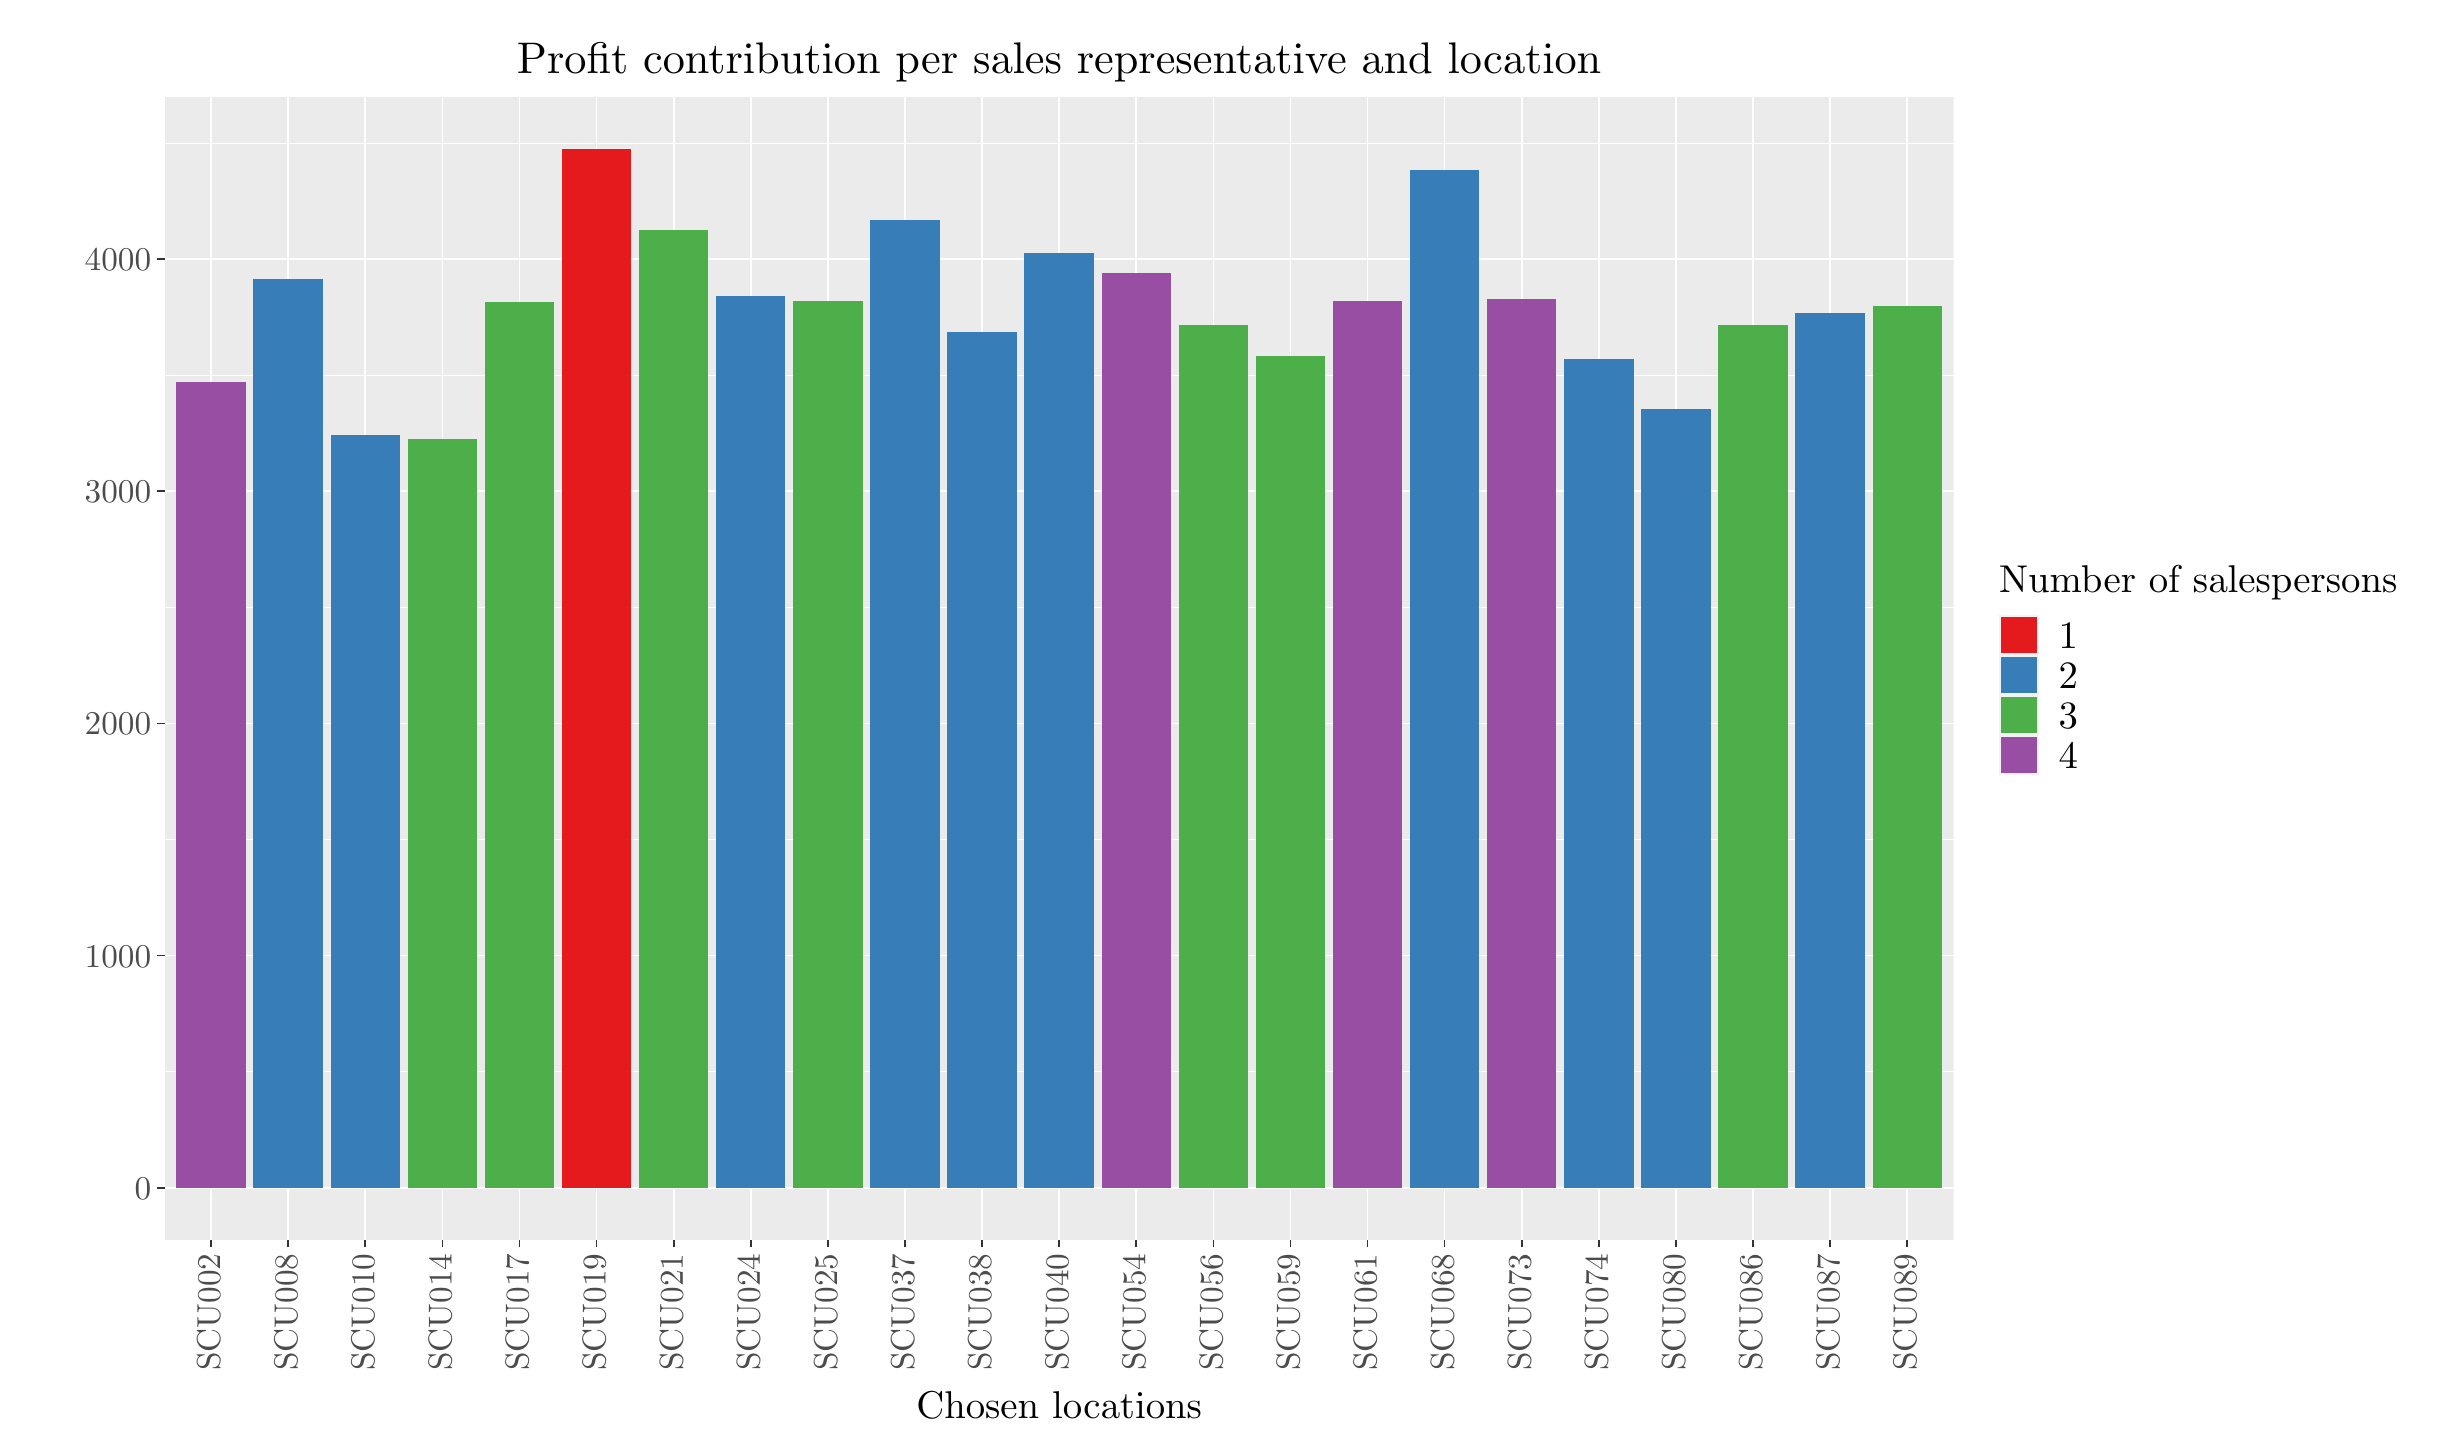
\begin{tikzpicture}[x=1pt,y=1pt]
\definecolor{fillColor}{RGB}{255,255,255}
\path[use as bounding box,fill=fillColor,fill opacity=0.00] (0,0) rectangle (867.24,505.89);
\begin{scope}
\path[clip] (  0.00,  0.00) rectangle (867.24,505.89);
\definecolor{drawColor}{RGB}{255,255,255}
\definecolor{fillColor}{RGB}{255,255,255}

\path[draw=drawColor,line width= 0.6pt,line join=round,line cap=round,fill=fillColor] ( -0.00,  0.00) rectangle (867.24,505.89);
\end{scope}
\begin{scope}
\path[clip] ( 49.56, 67.89) rectangle (695.89,480.76);
\definecolor{fillColor}{gray}{0.92}

\path[fill=fillColor] ( 49.56, 67.89) rectangle (695.89,480.76);
\definecolor{drawColor}{RGB}{255,255,255}

\path[draw=drawColor,line width= 0.3pt,line join=round] ( 49.56,128.61) --
	(695.89,128.61);

\path[draw=drawColor,line width= 0.3pt,line join=round] ( 49.56,212.51) --
	(695.89,212.51);

\path[draw=drawColor,line width= 0.3pt,line join=round] ( 49.56,296.42) --
	(695.89,296.42);

\path[draw=drawColor,line width= 0.3pt,line join=round] ( 49.56,380.32) --
	(695.89,380.32);

\path[draw=drawColor,line width= 0.3pt,line join=round] ( 49.56,464.23) --
	(695.89,464.23);

\path[draw=drawColor,line width= 0.6pt,line join=round] ( 49.56, 86.65) --
	(695.89, 86.65);

\path[draw=drawColor,line width= 0.6pt,line join=round] ( 49.56,170.56) --
	(695.89,170.56);

\path[draw=drawColor,line width= 0.6pt,line join=round] ( 49.56,254.46) --
	(695.89,254.46);

\path[draw=drawColor,line width= 0.6pt,line join=round] ( 49.56,338.37) --
	(695.89,338.37);

\path[draw=drawColor,line width= 0.6pt,line join=round] ( 49.56,422.27) --
	(695.89,422.27);

\path[draw=drawColor,line width= 0.6pt,line join=round] ( 66.27, 67.89) --
	( 66.27,480.76);

\path[draw=drawColor,line width= 0.6pt,line join=round] ( 94.13, 67.89) --
	( 94.13,480.76);

\path[draw=drawColor,line width= 0.6pt,line join=round] (121.99, 67.89) --
	(121.99,480.76);

\path[draw=drawColor,line width= 0.6pt,line join=round] (149.85, 67.89) --
	(149.85,480.76);

\path[draw=drawColor,line width= 0.6pt,line join=round] (177.71, 67.89) --
	(177.71,480.76);

\path[draw=drawColor,line width= 0.6pt,line join=round] (205.57, 67.89) --
	(205.57,480.76);

\path[draw=drawColor,line width= 0.6pt,line join=round] (233.43, 67.89) --
	(233.43,480.76);

\path[draw=drawColor,line width= 0.6pt,line join=round] (261.29, 67.89) --
	(261.29,480.76);

\path[draw=drawColor,line width= 0.6pt,line join=round] (289.15, 67.89) --
	(289.15,480.76);

\path[draw=drawColor,line width= 0.6pt,line join=round] (317.00, 67.89) --
	(317.00,480.76);

\path[draw=drawColor,line width= 0.6pt,line join=round] (344.86, 67.89) --
	(344.86,480.76);

\path[draw=drawColor,line width= 0.6pt,line join=round] (372.72, 67.89) --
	(372.72,480.76);

\path[draw=drawColor,line width= 0.6pt,line join=round] (400.58, 67.89) --
	(400.58,480.76);

\path[draw=drawColor,line width= 0.6pt,line join=round] (428.44, 67.89) --
	(428.44,480.76);

\path[draw=drawColor,line width= 0.6pt,line join=round] (456.30, 67.89) --
	(456.30,480.76);

\path[draw=drawColor,line width= 0.6pt,line join=round] (484.16, 67.89) --
	(484.16,480.76);

\path[draw=drawColor,line width= 0.6pt,line join=round] (512.02, 67.89) --
	(512.02,480.76);

\path[draw=drawColor,line width= 0.6pt,line join=round] (539.88, 67.89) --
	(539.88,480.76);

\path[draw=drawColor,line width= 0.6pt,line join=round] (567.74, 67.89) --
	(567.74,480.76);

\path[draw=drawColor,line width= 0.6pt,line join=round] (595.59, 67.89) --
	(595.59,480.76);

\path[draw=drawColor,line width= 0.6pt,line join=round] (623.45, 67.89) --
	(623.45,480.76);

\path[draw=drawColor,line width= 0.6pt,line join=round] (651.31, 67.89) --
	(651.31,480.76);

\path[draw=drawColor,line width= 0.6pt,line join=round] (679.17, 67.89) --
	(679.17,480.76);
\definecolor{fillColor}{RGB}{152,78,163}

\path[fill=fillColor] ( 53.74, 86.65) rectangle ( 78.81,377.78);
\definecolor{fillColor}{RGB}{55,126,184}

\path[fill=fillColor] ( 81.60, 86.65) rectangle (106.67,414.93);

\path[fill=fillColor] (109.45, 86.65) rectangle (134.53,358.82);
\definecolor{fillColor}{RGB}{77,175,74}

\path[fill=fillColor] (137.31, 86.65) rectangle (162.39,357.36);

\path[fill=fillColor] (165.17, 86.65) rectangle (190.25,406.66);
\definecolor{fillColor}{RGB}{228,26,28}

\path[fill=fillColor] (193.03, 86.65) rectangle (218.10,461.99);
\definecolor{fillColor}{RGB}{77,175,74}

\path[fill=fillColor] (220.89, 86.65) rectangle (245.96,432.61);
\definecolor{fillColor}{RGB}{55,126,184}

\path[fill=fillColor] (248.75, 86.65) rectangle (273.82,408.80);
\definecolor{fillColor}{RGB}{77,175,74}

\path[fill=fillColor] (276.61, 86.65) rectangle (301.68,406.94);
\definecolor{fillColor}{RGB}{55,126,184}

\path[fill=fillColor] (304.47, 86.65) rectangle (329.54,436.26);

\path[fill=fillColor] (332.33, 86.65) rectangle (357.40,395.91);

\path[fill=fillColor] (360.19, 86.65) rectangle (385.26,424.63);
\definecolor{fillColor}{RGB}{152,78,163}

\path[fill=fillColor] (388.04, 86.65) rectangle (413.12,417.22);
\definecolor{fillColor}{RGB}{77,175,74}

\path[fill=fillColor] (415.90, 86.65) rectangle (440.98,398.48);

\path[fill=fillColor] (443.76, 86.65) rectangle (468.84,387.09);
\definecolor{fillColor}{RGB}{152,78,163}

\path[fill=fillColor] (471.62, 86.65) rectangle (496.69,406.99);
\definecolor{fillColor}{RGB}{55,126,184}

\path[fill=fillColor] (499.48, 86.65) rectangle (524.55,454.36);
\definecolor{fillColor}{RGB}{152,78,163}

\path[fill=fillColor] (527.34, 86.65) rectangle (552.41,407.95);
\definecolor{fillColor}{RGB}{55,126,184}

\path[fill=fillColor] (555.20, 86.65) rectangle (580.27,386.22);

\path[fill=fillColor] (583.06, 86.65) rectangle (608.13,367.93);
\definecolor{fillColor}{RGB}{77,175,74}

\path[fill=fillColor] (610.92, 86.65) rectangle (635.99,398.39);
\definecolor{fillColor}{RGB}{55,126,184}

\path[fill=fillColor] (638.78, 86.65) rectangle (663.85,402.80);
\definecolor{fillColor}{RGB}{77,175,74}

\path[fill=fillColor] (666.63, 86.65) rectangle (691.71,405.41);
\end{scope}
\begin{scope}
\path[clip] (  0.00,  0.00) rectangle (867.24,505.89);
\definecolor{drawColor}{gray}{0.30}

\node[text=drawColor,anchor=base east,inner sep=0pt, outer sep=0pt, scale=  1.20] at ( 44.61, 82.52) {0};

\node[text=drawColor,anchor=base east,inner sep=0pt, outer sep=0pt, scale=  1.20] at ( 44.61,166.43) {1000};

\node[text=drawColor,anchor=base east,inner sep=0pt, outer sep=0pt, scale=  1.20] at ( 44.61,250.33) {2000};

\node[text=drawColor,anchor=base east,inner sep=0pt, outer sep=0pt, scale=  1.20] at ( 44.61,334.24) {3000};

\node[text=drawColor,anchor=base east,inner sep=0pt, outer sep=0pt, scale=  1.20] at ( 44.61,418.14) {4000};
\end{scope}
\begin{scope}
\path[clip] (  0.00,  0.00) rectangle (867.24,505.89);
\definecolor{drawColor}{gray}{0.20}

\path[draw=drawColor,line width= 0.6pt,line join=round] ( 46.81, 86.65) --
	( 49.56, 86.65);

\path[draw=drawColor,line width= 0.6pt,line join=round] ( 46.81,170.56) --
	( 49.56,170.56);

\path[draw=drawColor,line width= 0.6pt,line join=round] ( 46.81,254.46) --
	( 49.56,254.46);

\path[draw=drawColor,line width= 0.6pt,line join=round] ( 46.81,338.37) --
	( 49.56,338.37);

\path[draw=drawColor,line width= 0.6pt,line join=round] ( 46.81,422.27) --
	( 49.56,422.27);
\end{scope}
\begin{scope}
\path[clip] (  0.00,  0.00) rectangle (867.24,505.89);
\definecolor{drawColor}{gray}{0.20}

\path[draw=drawColor,line width= 0.6pt,line join=round] ( 66.27, 65.14) --
	( 66.27, 67.89);

\path[draw=drawColor,line width= 0.6pt,line join=round] ( 94.13, 65.14) --
	( 94.13, 67.89);

\path[draw=drawColor,line width= 0.6pt,line join=round] (121.99, 65.14) --
	(121.99, 67.89);

\path[draw=drawColor,line width= 0.6pt,line join=round] (149.85, 65.14) --
	(149.85, 67.89);

\path[draw=drawColor,line width= 0.6pt,line join=round] (177.71, 65.14) --
	(177.71, 67.89);

\path[draw=drawColor,line width= 0.6pt,line join=round] (205.57, 65.14) --
	(205.57, 67.89);

\path[draw=drawColor,line width= 0.6pt,line join=round] (233.43, 65.14) --
	(233.43, 67.89);

\path[draw=drawColor,line width= 0.6pt,line join=round] (261.29, 65.14) --
	(261.29, 67.89);

\path[draw=drawColor,line width= 0.6pt,line join=round] (289.15, 65.14) --
	(289.15, 67.89);

\path[draw=drawColor,line width= 0.6pt,line join=round] (317.00, 65.14) --
	(317.00, 67.89);

\path[draw=drawColor,line width= 0.6pt,line join=round] (344.86, 65.14) --
	(344.86, 67.89);

\path[draw=drawColor,line width= 0.6pt,line join=round] (372.72, 65.14) --
	(372.72, 67.89);

\path[draw=drawColor,line width= 0.6pt,line join=round] (400.58, 65.14) --
	(400.58, 67.89);

\path[draw=drawColor,line width= 0.6pt,line join=round] (428.44, 65.14) --
	(428.44, 67.89);

\path[draw=drawColor,line width= 0.6pt,line join=round] (456.30, 65.14) --
	(456.30, 67.89);

\path[draw=drawColor,line width= 0.6pt,line join=round] (484.16, 65.14) --
	(484.16, 67.89);

\path[draw=drawColor,line width= 0.6pt,line join=round] (512.02, 65.14) --
	(512.02, 67.89);

\path[draw=drawColor,line width= 0.6pt,line join=round] (539.88, 65.14) --
	(539.88, 67.89);

\path[draw=drawColor,line width= 0.6pt,line join=round] (567.74, 65.14) --
	(567.74, 67.89);

\path[draw=drawColor,line width= 0.6pt,line join=round] (595.59, 65.14) --
	(595.59, 67.89);

\path[draw=drawColor,line width= 0.6pt,line join=round] (623.45, 65.14) --
	(623.45, 67.89);

\path[draw=drawColor,line width= 0.6pt,line join=round] (651.31, 65.14) --
	(651.31, 67.89);

\path[draw=drawColor,line width= 0.6pt,line join=round] (679.17, 65.14) --
	(679.17, 67.89);
\end{scope}
\begin{scope}
\path[clip] (  0.00,  0.00) rectangle (867.24,505.89);
\definecolor{drawColor}{gray}{0.30}

\node[text=drawColor,rotate= 90.00,anchor=base east,inner sep=0pt, outer sep=0pt, scale=  1.20] at ( 69.58, 62.94) {SCU002};

\node[text=drawColor,rotate= 90.00,anchor=base east,inner sep=0pt, outer sep=0pt, scale=  1.20] at ( 97.44, 62.94) {SCU008};

\node[text=drawColor,rotate= 90.00,anchor=base east,inner sep=0pt, outer sep=0pt, scale=  1.20] at (125.30, 62.94) {SCU010};

\node[text=drawColor,rotate= 90.00,anchor=base east,inner sep=0pt, outer sep=0pt, scale=  1.20] at (153.16, 62.94) {SCU014};

\node[text=drawColor,rotate= 90.00,anchor=base east,inner sep=0pt, outer sep=0pt, scale=  1.20] at (181.01, 62.94) {SCU017};

\node[text=drawColor,rotate= 90.00,anchor=base east,inner sep=0pt, outer sep=0pt, scale=  1.20] at (208.87, 62.94) {SCU019};

\node[text=drawColor,rotate= 90.00,anchor=base east,inner sep=0pt, outer sep=0pt, scale=  1.20] at (236.73, 62.94) {SCU021};

\node[text=drawColor,rotate= 90.00,anchor=base east,inner sep=0pt, outer sep=0pt, scale=  1.20] at (264.59, 62.94) {SCU024};

\node[text=drawColor,rotate= 90.00,anchor=base east,inner sep=0pt, outer sep=0pt, scale=  1.20] at (292.45, 62.94) {SCU025};

\node[text=drawColor,rotate= 90.00,anchor=base east,inner sep=0pt, outer sep=0pt, scale=  1.20] at (320.31, 62.94) {SCU037};

\node[text=drawColor,rotate= 90.00,anchor=base east,inner sep=0pt, outer sep=0pt, scale=  1.20] at (348.17, 62.94) {SCU038};

\node[text=drawColor,rotate= 90.00,anchor=base east,inner sep=0pt, outer sep=0pt, scale=  1.20] at (376.03, 62.94) {SCU040};

\node[text=drawColor,rotate= 90.00,anchor=base east,inner sep=0pt, outer sep=0pt, scale=  1.20] at (403.89, 62.94) {SCU054};

\node[text=drawColor,rotate= 90.00,anchor=base east,inner sep=0pt, outer sep=0pt, scale=  1.20] at (431.75, 62.94) {SCU056};

\node[text=drawColor,rotate= 90.00,anchor=base east,inner sep=0pt, outer sep=0pt, scale=  1.20] at (459.61, 62.94) {SCU059};

\node[text=drawColor,rotate= 90.00,anchor=base east,inner sep=0pt, outer sep=0pt, scale=  1.20] at (487.46, 62.94) {SCU061};

\node[text=drawColor,rotate= 90.00,anchor=base east,inner sep=0pt, outer sep=0pt, scale=  1.20] at (515.32, 62.94) {SCU068};

\node[text=drawColor,rotate= 90.00,anchor=base east,inner sep=0pt, outer sep=0pt, scale=  1.20] at (543.18, 62.94) {SCU073};

\node[text=drawColor,rotate= 90.00,anchor=base east,inner sep=0pt, outer sep=0pt, scale=  1.20] at (571.04, 62.94) {SCU074};

\node[text=drawColor,rotate= 90.00,anchor=base east,inner sep=0pt, outer sep=0pt, scale=  1.20] at (598.90, 62.94) {SCU080};

\node[text=drawColor,rotate= 90.00,anchor=base east,inner sep=0pt, outer sep=0pt, scale=  1.20] at (626.76, 62.94) {SCU086};

\node[text=drawColor,rotate= 90.00,anchor=base east,inner sep=0pt, outer sep=0pt, scale=  1.20] at (654.62, 62.94) {SCU087};

\node[text=drawColor,rotate= 90.00,anchor=base east,inner sep=0pt, outer sep=0pt, scale=  1.20] at (682.48, 62.94) {SCU089};
\end{scope}
\begin{scope}
\path[clip] (  0.00,  0.00) rectangle (867.24,505.89);
\definecolor{drawColor}{RGB}{0,0,0}

\node[text=drawColor,anchor=base,inner sep=0pt, outer sep=0pt, scale=  1.40] at (372.72,  3.32) {Chosen locations};
\end{scope}
\begin{scope}
\path[clip] (  0.00,  0.00) rectangle (867.24,505.89);
\definecolor{fillColor}{RGB}{255,255,255}

\path[fill=fillColor] (706.89,230.23) rectangle (861.74,318.41);
\end{scope}
\begin{scope}
\path[clip] (  0.00,  0.00) rectangle (867.24,505.89);
\definecolor{drawColor}{RGB}{0,0,0}

\node[text=drawColor,anchor=base west,inner sep=0pt, outer sep=0pt, scale=  1.40] at (712.39,301.91) {Number of salespersons};
\end{scope}
\begin{scope}
\path[clip] (  0.00,  0.00) rectangle (867.24,505.89);
\definecolor{fillColor}{gray}{0.95}

\path[fill=fillColor] (712.39,279.10) rectangle (726.84,293.55);
\end{scope}
\begin{scope}
\path[clip] (  0.00,  0.00) rectangle (867.24,505.89);
\definecolor{fillColor}{RGB}{228,26,28}

\path[fill=fillColor] (713.10,279.81) rectangle (726.13,292.84);
\end{scope}
\begin{scope}
\path[clip] (  0.00,  0.00) rectangle (867.24,505.89);
\definecolor{fillColor}{gray}{0.95}

\path[fill=fillColor] (712.39,264.64) rectangle (726.84,279.10);
\end{scope}
\begin{scope}
\path[clip] (  0.00,  0.00) rectangle (867.24,505.89);
\definecolor{fillColor}{RGB}{55,126,184}

\path[fill=fillColor] (713.10,265.35) rectangle (726.13,278.38);
\end{scope}
\begin{scope}
\path[clip] (  0.00,  0.00) rectangle (867.24,505.89);
\definecolor{fillColor}{gray}{0.95}

\path[fill=fillColor] (712.39,250.19) rectangle (726.84,264.64);
\end{scope}
\begin{scope}
\path[clip] (  0.00,  0.00) rectangle (867.24,505.89);
\definecolor{fillColor}{RGB}{77,175,74}

\path[fill=fillColor] (713.10,250.90) rectangle (726.13,263.93);
\end{scope}
\begin{scope}
\path[clip] (  0.00,  0.00) rectangle (867.24,505.89);
\definecolor{fillColor}{gray}{0.95}

\path[fill=fillColor] (712.39,235.73) rectangle (726.84,250.19);
\end{scope}
\begin{scope}
\path[clip] (  0.00,  0.00) rectangle (867.24,505.89);
\definecolor{fillColor}{RGB}{152,78,163}

\path[fill=fillColor] (713.10,236.44) rectangle (726.13,249.48);
\end{scope}
\begin{scope}
\path[clip] (  0.00,  0.00) rectangle (867.24,505.89);
\definecolor{drawColor}{RGB}{0,0,0}

\node[text=drawColor,anchor=base west,inner sep=0pt, outer sep=0pt, scale=  1.40] at (733.84,281.50) {1};
\end{scope}
\begin{scope}
\path[clip] (  0.00,  0.00) rectangle (867.24,505.89);
\definecolor{drawColor}{RGB}{0,0,0}

\node[text=drawColor,anchor=base west,inner sep=0pt, outer sep=0pt, scale=  1.40] at (733.84,267.05) {2};
\end{scope}
\begin{scope}
\path[clip] (  0.00,  0.00) rectangle (867.24,505.89);
\definecolor{drawColor}{RGB}{0,0,0}

\node[text=drawColor,anchor=base west,inner sep=0pt, outer sep=0pt, scale=  1.40] at (733.84,252.59) {3};
\end{scope}
\begin{scope}
\path[clip] (  0.00,  0.00) rectangle (867.24,505.89);
\definecolor{drawColor}{RGB}{0,0,0}

\node[text=drawColor,anchor=base west,inner sep=0pt, outer sep=0pt, scale=  1.40] at (733.84,238.14) {4};
\end{scope}
\begin{scope}
\path[clip] (  0.00,  0.00) rectangle (867.24,505.89);
\definecolor{drawColor}{RGB}{0,0,0}

\node[text=drawColor,anchor=base,inner sep=0pt, outer sep=0pt, scale=  1.60] at (372.72,489.37) {Profit contribution per sales representative and location};
\end{scope}
\end{tikzpicture}

\end{document}